\section{Bootloader optimizations}

\subsection{Generic bootloader optimizations}

\begin{frame}
\frametitle{Bootloader}
\begin{itemize}

\item Remove unnecessary functionality.\\
      Usually, bootloaders include many features needed only for
      development. Compile your bootloader with fewer features.
\item Optimize required functionality.\\
      Tune your bootloader for fastest performance. \\
      Skip the bootloader and load the kernel right away.
\end{itemize}
\end{frame}

\begin{frame}
\frametitle{U-Boot - Remove unnecessary functionality}
Recompile U-Boot to remove features not needed in production
\begin{itemize}
\item Disable as many features as possible
      in \code{include/configs/<soc>-<board>.h}
\item Examples: MMC, USB, Ethernet, dhcp, ping, command line edition,
      command completion...
\item A smaller and simpler U-Boot is faster to load and faster
      to initialize.
\end{itemize}
\end{frame}

\begin{frame}
\frametitle{U-Boot - Remove the boot delay}
\begin{itemize}
\item Remove the boot delay:\\
      \code{setenv bootdelay 0}
\item This usually saves several seconds!
\end{itemize}
\end{frame}

\begin{frame}[fragile]
\frametitle{U-Boot - Simplify scripts}
Some boards have over-complicated scripts:
\begin{center}
    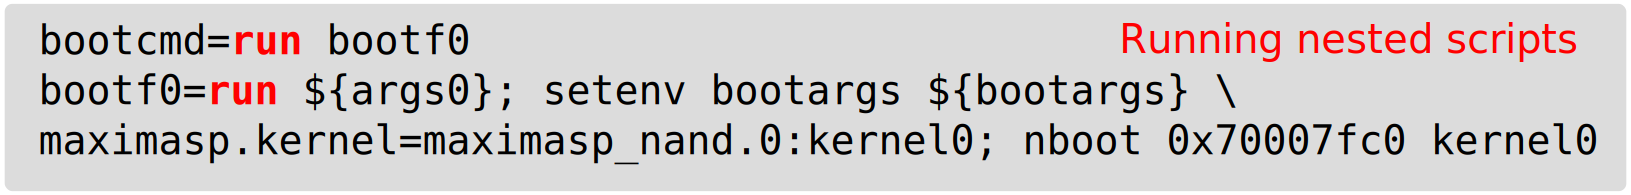
\includegraphics[width=\textwidth]{slides/boot-time-bootloader/u-boot-bad-scripts.pdf}
\end{center}
Let's replace this by:
\begin{block}{}
\footnotesize
\begin{verbatim}
setenv bootargs 'mem=128M console=tty0 consoleblank=0
console=ttyS0,57600 \
mtdparts=maximasp_nand.0:2M(u-boot)ro,512k(env0)ro,512k(env1)ro,\
4M(kernel0),4M(kernel1),5M(kernel2),100M(root0),100M(root1),-(other)\
rw ubi.mtd=root0 root=ubi0:rootfs rootfstype=ubifs earlyprintk debug \
user_debug=28 maximasp.board=EEKv1.3.x \
maximasp.kernel=maximasp_nand.0:kernel0'
setenv bootcmd 'nboot 0x70007fc0 kernel0'
\end{verbatim}
\end{block}
This saved 56 ms on this ARM9 system (400 MHz)!
\end{frame}

\begin{frame}
\frametitle{Bootloader: copy the exact kernel size}
\begin{itemize}
\item When copying the kernel from {\bf raw} flash to RAM, we still see
      many systems that copy too many bytes, not taking the
      exact kernel size into account.
\item A solution is to store the exact size of the kernel in an environment
      variable, and use it a kernel loading time.
\item Of course, that's not needed when the kernel is loaded from a
      filesystem, which knows how big the file is.
\end{itemize}
\end{frame}

\begin{frame}
\frametitle{U-Boot - Optimize kernel loading}
\begin{itemize}
\item After copying the kernel \code{uImage} to RAM,
      U-Boot always moves it to the load address specified
      in the \code{uImage} header.
\item A CRC check is also performed.
\end{itemize}
\begin{center}
    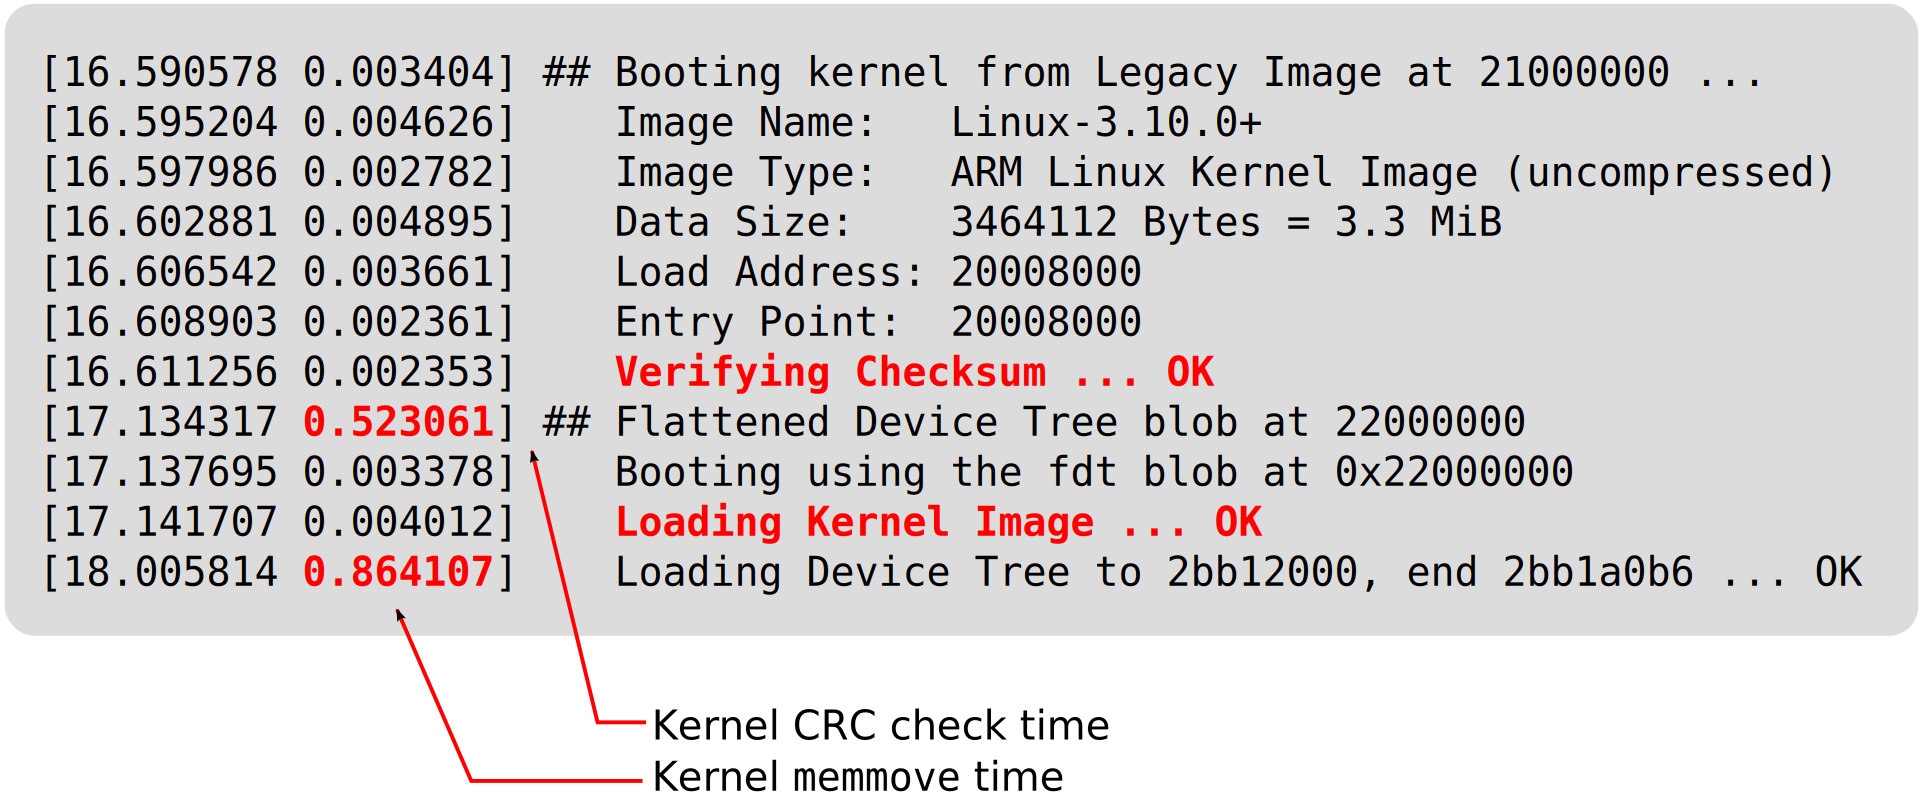
\includegraphics[width=\textwidth]{slides/boot-time-bootloader/u-boot-kernel-loading.pdf}
\end{center}
\end{frame}

\begin{frame}
\frametitle{U-Boot - Remove unnecessary memmove (1)}
\begin{itemize}
\item You can make U-Boot skip the \code{memmove} operation
      by directly loading the \code{uImage} at the right
      address.
\item Compute this address: \\
      {\small
      \code{Addr = Load Address - uImage header size}\\
      \code{Addr = Load Address - (size(uImage) - size(zImage))}\\
      \code{Addr = 0x20008000 - 0x40 = 0x20007fc0}\\
      }
\end{itemize}
\begin{center}
    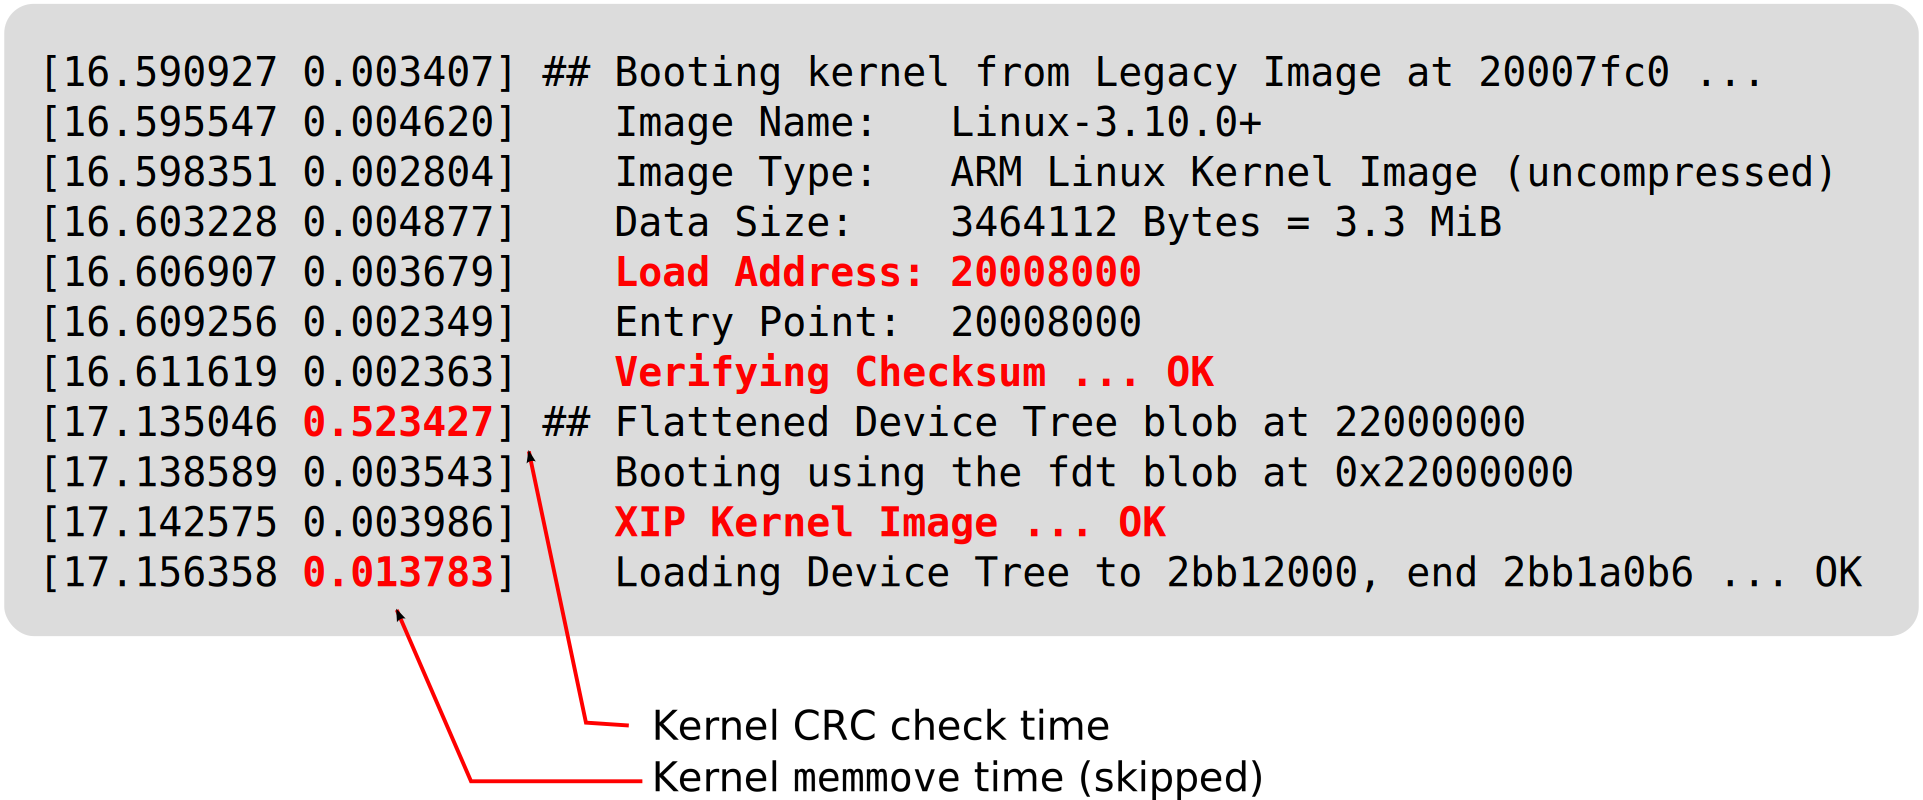
\includegraphics[height=0.5\textheight]{slides/boot-time-bootloader/u-boot-kernel-loading-no-memmove.pdf}
\end{center}
\end{frame}

\begin{frame}
\frametitle{U-Boot - Remove unnecessary memmove (2)}
Results on Microchip SAMA5D3 Xplained (ARM), Linux 3.10:
\newline\newline
\begin{tabular}{| l || c | c |}
\hline
& Time & Diff \\
\hline
Default & 1.433 s & \\
Optimum load address & 0.583 s & -0.85 s\\
\hline
\end{tabular}
\newline\newline
\small
Measured between \code{Booting kernel} and \code{Starting kernel ...}
\end{frame}

\begin{frame}
\frametitle{U-Boot - Remove kernel CRC check}
\begin{itemize}
\item Fine in production when you never have data corruption
      copying the kernel to RAM.
\item Disable CRC checking with a U-boot environment variable:\\
      \code{setenv verify no}
\end{itemize}
Results on Microchip SAMA5D3 Xplained (ARM), Linux 3.10:
\newline\newline
\begin{tabular}{| l || c | c |}
\hline
& Time & Diff \\
\hline
With CRC check & 583 ms & \\
Without CRC check & 60 ms & -523 ms \\
\hline
\end{tabular}
\newline\newline
\small
Measured between \code{Booting kernel} and \code{Starting kernel ...}
\end{frame}

\begin{frame}
\frametitle{Further U-Boot optimizations}
\begin{itemize}
\item Silence U-Boot console output. You will need to compile
      U-Boot with \projconfig{u-boot}{CONFIG_SILENT_CONSOLE} and
      \code{setenv silent yes}.\\
      See \projfile{u-boot}{doc/README.silent} for details.
\end{itemize}
\end{frame}
